\documentclass[english, 12pt, a4paper]{article}
\usepackage[utf8]{inputenc}
\usepackage[T1]{fontenc}
\usepackage{mwe,tikz}
\usepackage{color}
\usepackage{xcolor}
\usepackage{amssymb}
\usepackage[most]{tcolorbox}
\usepackage{colortbl}
\usepackage{pgfplots}

\begin{document}

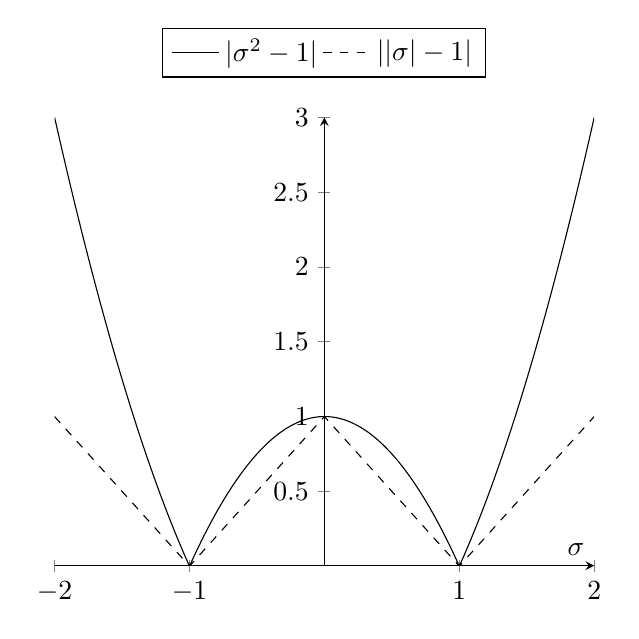
\begin{tikzpicture}
\begin{axis}[
    axis lines = center,
    xlabel = $\sigma$,
    legend style={at={(0.5,1.2)}, anchor=north,legend columns=-1}
]

\addplot [
    domain=-2:2, 
    samples=300, 
    color=black,
    ]
    {abs(x^2 -1)};
\addlegendentry{$|\sigma^2 -1|$}
\addplot [dashed,
    domain=-2:2, 
    samples=300, 
    color=black,
]
{abs(abs(x)-1)};
\addlegendentry{$||\sigma| -1|$}
\end{axis}
\end{tikzpicture}

\end{document}